\documentclass{article}

\usepackage[T1]{fontenc}
\usepackage{lmodern}
\usepackage{tikz}
\usepackage{framed}
\usepackage[hmargin = 0.8in]{geometry}
\usetikzlibrary{arrows.meta, automata, positioning}

\title{Automaton}
\author{}
\date{}

\begin{document}

\begin{center}

    \section*{Finite--State Automaton for the Parser}
    \vspace{0.3in}

\begin{framed}
    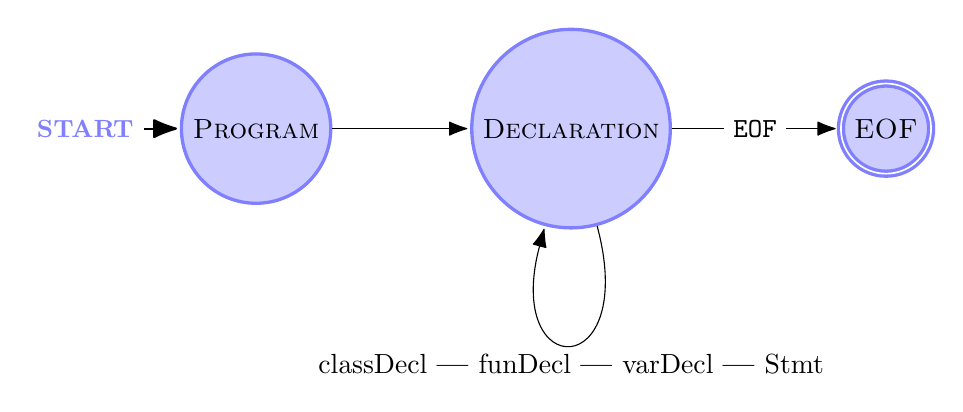
\begin{tikzpicture}[
        shorten >= 1pt, 
        node distance = 4cm,
        on grid, 
        >= {Latex[round, scale = 1.5]},
        every state/.style = {draw = blue!50, very thick, fill = blue!20},
        every initial by arrow/.style = {text = blue!50, draw = black, thick}
    ]

      \node[state, initial, 
            initial where = left,
            initial text = {\small\textbf{START}} 
      ] (s_0) {\textsc{Program}};

      \node[state] (s_1)            [right = of s_0] {\textsc{Declaration}};
      \node[state, accepting] (s_e) [right = of s_1] {\textsc{EOF}};

      \path[->] (s_0) edge []             node {}    (s_1)
                (s_1) edge [fill = white] node [fill = white] {\texttt{\textbf{EOF}}} (s_e)
                (s_1) edge [loop below]   node {classDecl \textbf{|} funDecl \textbf{|} varDecl \textbf{|} Stmt} (s_1);

    \end{tikzpicture}
\end{framed}


    \vspace{0.3in}
    \section*{Declaration}
    \vspace{0.3in}

\begin{framed}
    \begin{tikzpicture}[
        shorten >= 1pt, 
        node distance = 4cm,
        on grid, 
        >= {Latex[round, scale = 1.5]},
        every state/.style = {draw = blue!50, very thick, fill = blue!20},
        every initial by arrow/.style = {text = blue!50, draw = black, thick}
    ]


    \node[state] (decl) [] {\textbf{START}};

    \node[state] (class) [above left = of decl]  {classDecl};
    \node[state] (def)   [above right = of decl] {funDecl};
    \node[state] (var)   [below left = of decl]  {varDecl};
    \node[state] (stmt)  [below right = of decl] {Stmt};
    \node[state, accepting] (s_e) [right = 2cm of s_1] {\textsc{EOF}};

    \path[->]
        
        (decl) edge [bend left]  node [fill = white] {\textbf{\texttt{`class'}}}    (class)
        (decl) edge [bend right] node [fill = white] {\textbf{\texttt{`def'}}}      (def)
        (decl) edge [bend right] node [fill = white] {\textbf{\texttt{`var'}}}      (var)
        (decl) edge [bend left]  node [fill = white] {\textbf{\texttt{\Large *}}} (stmt)
        (decl) edge [left = of decl] node [fill = white] {\textbf{\texttt{EOF}}}     (s_e);

    \path[->]

        (class) edge [bend left]  node [fill = white] {\textbf{\texttt{\Large `\}'}}} (decl)
        (def)   edge [bend right] node [fill = white] {\textbf{\texttt{\Large `\}'}}} (decl)
        (var)   edge [bend right] node [fill = white] {\textbf{\texttt{\Large `;'}}}  (decl)
        (stmt)  edge [bend left]  node [fill = white] {\textbf{\texttt{\Large `;'}}}  (decl);




    \end{tikzpicture}
\end{framed}


    \pagebreak



    \section*{Class Declaration}
    \vspace{0.001in}
        

\begin{framed}
    

    
    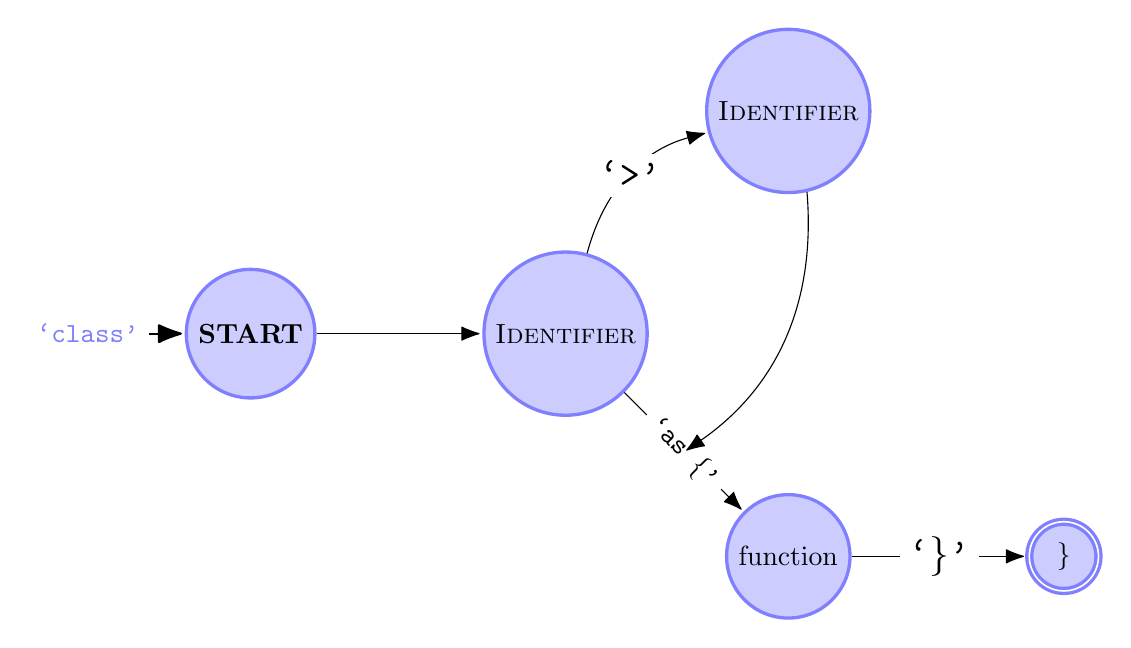
\begin{tikzpicture}[
        shorten >= 1pt, 
        node distance = 4cm,
        on grid, 
        >= {Latex[round, scale = 1.5]},
        every state/.style = {draw = blue!50, very thick, fill = blue!20},
        every initial by arrow/.style = {text = blue!50, draw = black, thick}
    ]


      \node[state, initial, 
            initial where = left,
            initial text = {\textbf{\texttt{`class'}}} 
      ] (decl) {\textbf{START}};

      \node[state] (name) [right of = decl] {\textsc{Identifier}};
      \node[state] (super) [above right of = name] {\textsc{Identifier}};
      \node[state] (func) [below right of = name] {function};

      \node[state, accepting] (s_e) [right = 3.5cm of func] {\texttt{\textbf{\}}}};


      \path[->]

            (decl) edge [right] node [] {} (name)
            (name) edge [bend left] node [fill = white] {\Large \textbf{\texttt{`>'}}} (super)
            (name) edge [sloped, below right = 1.7cm of name] node [fill = white] {\textbf{\texttt{`as \{'}}} coordinate (junction) (func)
            (func) edge [right of = func] node [fill = white] {\Large \textbf{\texttt{`\}'}}} (s_e)
    
    (super) edge [bend left] (junction);



    \end{tikzpicture}


\end{framed}


    
    \vspace{0.05in}
    \section*{Function Declaration}
    \vspace{0.01in}


\begin{framed}
    


    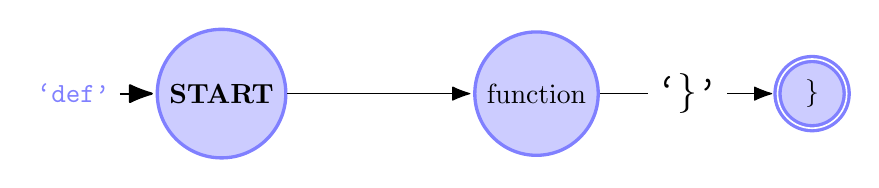
\begin{tikzpicture}[
        shorten >= 1pt, 
        node distance = 4cm,
        on grid, 
        >= {Latex[round, scale = 1.5]},
        every state/.style = {draw = blue!50, very thick, fill = blue!20},
        every initial by arrow/.style = {text = blue!50, draw = black, thick}
    ]


      \node[state, initial, 
            initial where = left,
            initial text = {\textbf{\texttt{`def'}}} 
      ] (decl) {\textbf{START}};

      \node[state] (func) [right of = decl] {function};
      \node[state, accepting] (s_e) [right = 3.5cm of func] {\texttt{\textbf{\}}}};


      \path[->]

            (decl) edge [right of = decl] node [] {} (func)
            (func) edge [right of = func] node [fill = white] {\Large \textbf{\texttt{`\}'}}} (s_e);

    \end{tikzpicture}

\end{framed}


    \pagebreak


    \section*{Variable Declaration}


\begin{framed}
    


    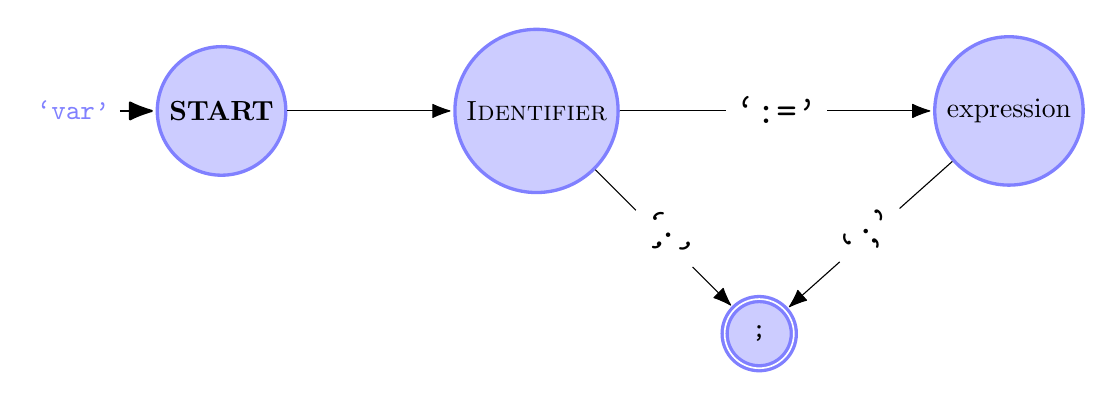
\begin{tikzpicture}[
        shorten >= 1pt, 
        node distance = 4cm,
        on grid, 
        >= {Latex[round, scale = 1.5]},
        every state/.style = {draw = blue!50, very thick, fill = blue!20},
        every initial by arrow/.style = {text = blue!50, draw = black, thick}
    ]


    
      \node[state, initial, 
            initial where = left,
            initial text = {\textbf{\texttt{`var'}}} 
      ] (decl) {\textbf{START}};

        
      \node[state] (name) [right of = decl] {\textsc{Identifier}};
      \node[state] (expr) [right = 6cm of name] {expression};
      \node[state, accepting] (s_e) [below right of = name] {\texttt{\textbf{;}}};


      \path[->]

            (decl) edge [right of = decl] node [] {} (name)
            (name) edge [right of = name] node [fill = white] {\Large \textbf{\texttt{`:='}}} (expr)
            (name) edge [sloped] node [fill = white] {\Large \texttt{\textbf{`;'}}} (s_e)
            (expr) edge [sloped] node [fill = white] {\Large \texttt{\textbf{`;'}}} (s_e);
            



    \end{tikzpicture}
\end{framed}

\pagebreak


    \section*{Statements}



\begin{framed}

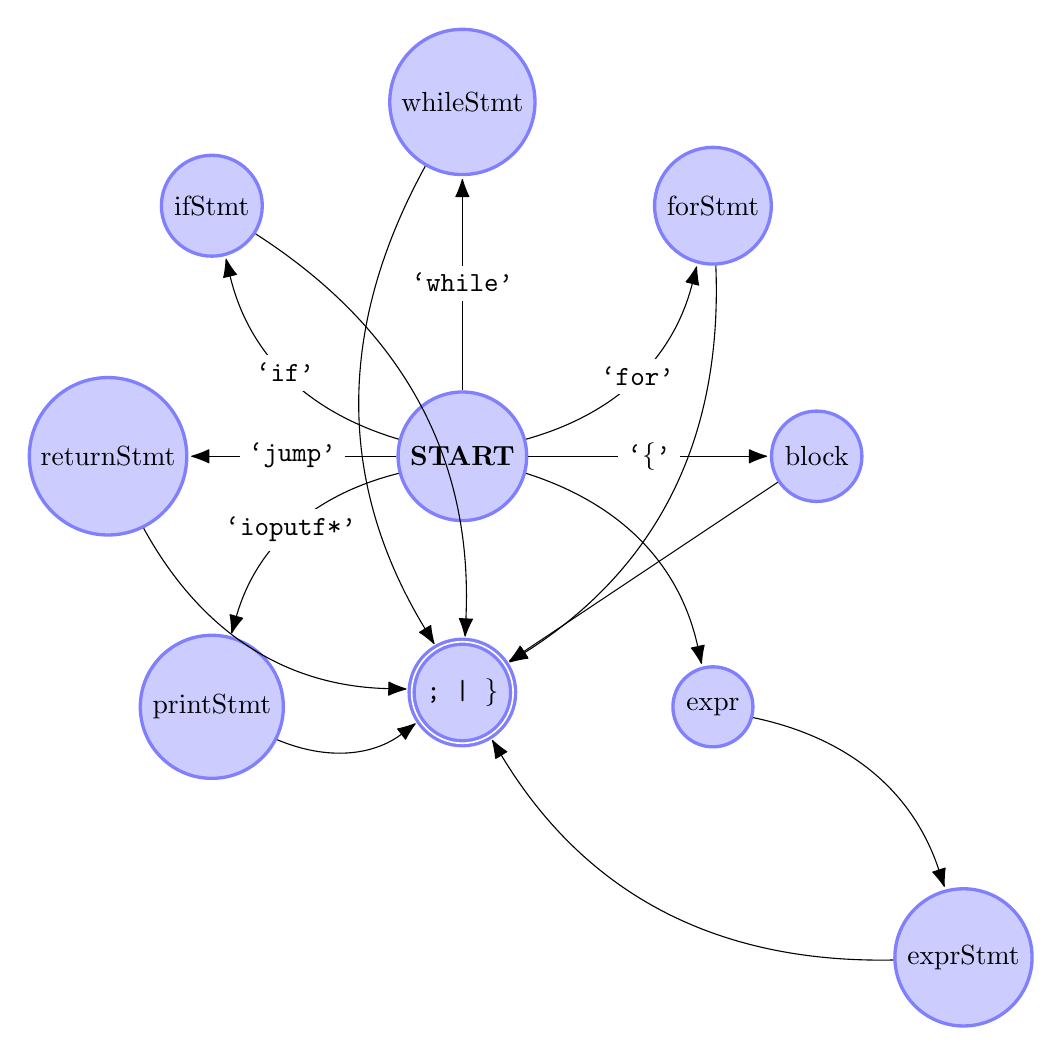
\begin{tikzpicture}[
        shorten >= 1pt, 
        node distance = 4.5cm,
        on grid, 
        >= {Latex[round, scale = 1.5]},
        every state/.style = {draw = blue!50, very thick, fill = blue!20},
        every initial by arrow/.style = {text = blue!50, draw = black, thick}
    ]

    \node[state] (start) {\textbf{START}};

    \node[state] (if)     [above left = of start]  {ifStmt};
    \node[state] (while)  [above = of start]       {whileStmt};
    \node[state] (for)    [above right = of start] {forStmt};

    \node[state] (jump)   [left = of start]        {returnStmt};
    \node[state] (block)  [right = of start]       {block};

    \node[state] (io)     [below left = of start]  {printStmt};

    \node[state] (_expr)  [below right = of start] {expr};
    \node[state] (expr)   [below right = of _expr] {exprStmt};

    \node[state, accepting] (end) [below = 3cm of start] {\texttt{\textbf{; | \}}}};

    \path[->]
        (start) edge [bend left]  node [fill = white] {\texttt{`if'}}         (if)
        (start) edge []           node [fill = white] {\texttt{`while'}}      (while)
        (start) edge [bend right] node [fill = white] {\texttt{`for'}}        (for)
        (start) edge []           node [fill = white] {\texttt{`jump'}}       (jump)
        (start) edge []           node [fill = white] {\texttt{`\{'}}          (block)
        (start) edge [bend right] node [fill = white] {\texttt{`ioputf*'}}     (io)
        (start) edge [bend left]  node [] {}   (_expr)
        (_expr) edge [bend left]  node [] {}   (expr);

    \path[->]
        (if)     edge [bend left]  node {} (end)
        (while)  edge [bend right] node {} (end)
        (for)    edge [bend left]  node {} (end)
        (jump)   edge [bend right] node {} (end)
        (block)  edge []           node {} (end)
        (io)     edge [bend right] node {} (end)
        (expr)   edge [bend left]  node {} (end);

    \end{tikzpicture}


\end{framed}


    \section*{Expression Statement}
    \begin{framed}
    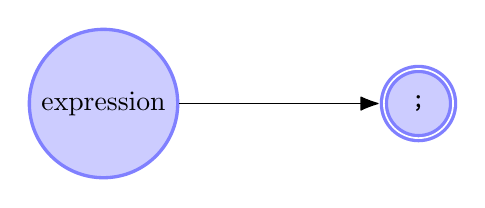
\begin{tikzpicture}[
        shorten >= 1pt, node distance = 4cm, on grid, 
        >= {Latex[round, scale = 1.5]},
        every state/.style = {draw = blue!50, very thick, fill = blue!20},
        every initial by arrow/.style = {text = blue!50, draw = black, thick}
    ]
      \node[state] (exp) {expression};
      \node[state, accepting] (s_e) [right = of exp] {\texttt{\textbf{;}}};

      \path[->] (exp) edge node [] {} (s_e);
    \end{tikzpicture}
    \end{framed}

    \section*{If Statement}
    \begin{framed}
    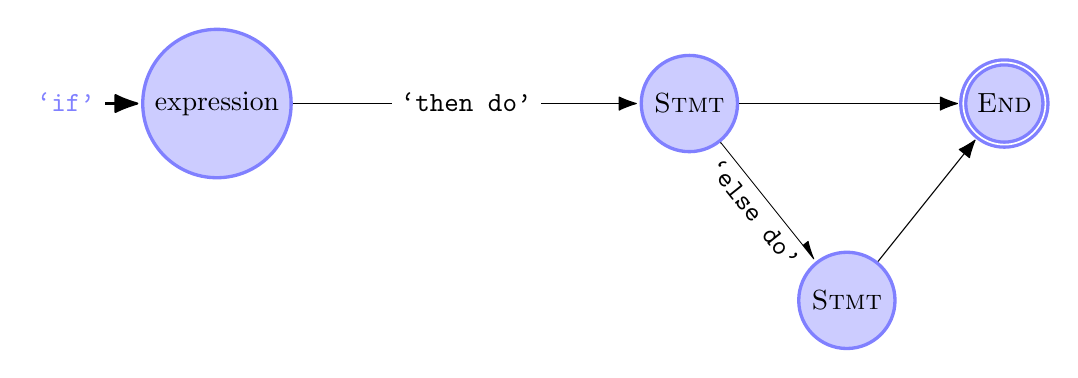
\begin{tikzpicture}[
        shorten >= 1pt, node distance = 3.5cm, on grid, 
        >= {Latex[round, scale = 1.5]},
        every state/.style = {draw = blue!50, very thick, fill = blue!20},
        every initial by arrow/.style = {text = blue!50, draw = black, thick}
    ]
      \node[state, initial, initial where = left, initial text = {\textbf{\texttt{`if'}}}] (exp) {expression};
        \node[state] (then) [right = 6cm of exp] {\textsc{Stmt}};
      \node[state, accepting] (s_e) [right = 4cm of then] {\textsc{End}};
      \node[state] (else) [below right = 2.5cm and 2cm of then] {\textsc{Stmt}};

      \path[->] 
        (exp)   edge node [fill = white] {\texttt{`then do'}} (then)
        (then)  edge node {} (s_e)
        (then)  edge [sloped, below] node [fill = white] {\texttt{`else do'}} (else)
        (else)  edge [sloped, above] node {} (s_e);
    \end{tikzpicture}
    \end{framed}

    \section*{While Statement}
    \begin{framed}
    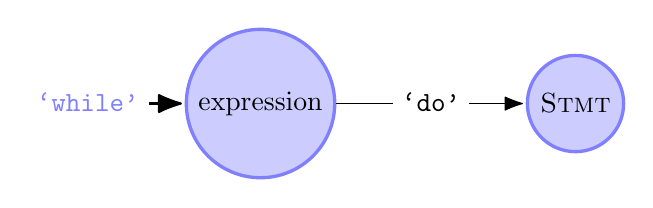
\begin{tikzpicture}[
        shorten >= 1pt, node distance = 4cm, on grid, 
        >= {Latex[round, scale = 1.5]},
        every state/.style = {draw = blue!50, very thick, fill = blue!20},
        every initial by arrow/.style = {text = blue!50, draw = black, thick}
    ]
      \node[state, initial, initial where = left, initial text = {\textbf{\texttt{`while'}}}] (exp) {expression};
        \node[state] (stmt) [right = of exp] {\textsc{Stmt}};

      \path[->] 
        (exp) edge node [fill = white] {\texttt{`do'}} (stmt);
    \end{tikzpicture}
    \end{framed}

    \section*{For Statement}
    \begin{framed}
    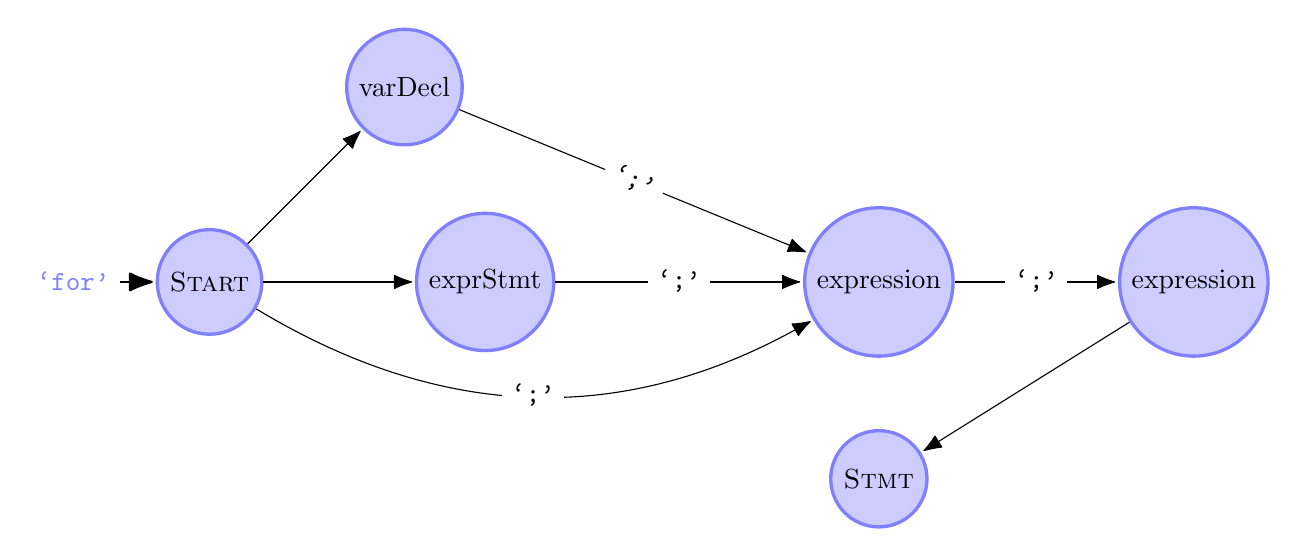
\begin{tikzpicture}[
        shorten >= 1pt, node distance = 3.5cm, on grid, 
        >= {Latex[round, scale = 1.5]},
        every state/.style = {draw = blue!50, very thick, fill = blue!20},
        every initial by arrow/.style = {text = blue!50, draw = black, thick}
    ]
        \node[state, initial, initial where = left, initial text = {\textbf{\texttt{`for'}}}] (init) {\textsc{Start}};
        \node[state] (varDecl) [above right = of init] {varDecl};
        \node[state] (exprStmt) [right = of init] {exprStmt};
      \node[state] (cond) [right = 5cm of exprStmt] {expression};
      \node[state] (incr) [right = 4cm of cond] {expression};
        \node[state] (stmt) [below = 2.5cm of cond] {\textsc{Stmt}};
      

      \path[->] 
        (init) edge [sloped, above]  node [] {} (varDecl)
        (init) edge []           node [] {} (exprStmt)
        (varDecl) edge [sloped] node [fill = white] {\texttt{`;'}} (cond)
        (exprStmt) edge [] node [fill = white] {\texttt{`;'}} (cond)
        (init) edge [bend right] node [fill = white] {\texttt{`;'}} (cond)
        (cond) edge node [fill = white] {\texttt{`;'}} (incr)
        (incr) edge [sloped, below] node {} (stmt);
    \end{tikzpicture}
    \end{framed}

    \pagebreak

    \section*{Return Statement}
    \begin{framed}
    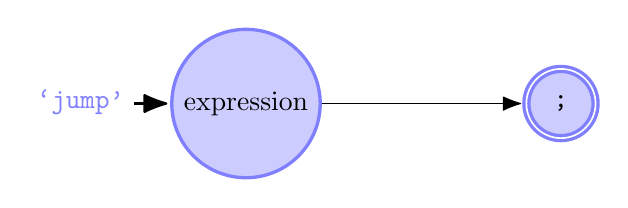
\begin{tikzpicture}[
        shorten >= 1pt, node distance = 4cm, on grid, 
        >= {Latex[round, scale = 1.5]},
        every state/.style = {draw = blue!50, very thick, fill = blue!20},
        every initial by arrow/.style = {text = blue!50, draw = black, thick}
    ]
      \node[state, initial, initial text = {\textbf{\texttt{`jump'}}}] (ret) {expression};
      \node[state, accepting] (s_e1) [right = of ret] {\texttt{\textbf{;}}};
      
      \path[->] (ret) edge node {} (s_e1);
    \end{tikzpicture}
    \end{framed}


    \section*{Print Statement}
    \begin{framed}
    \begin{tikzpicture}[
        shorten >= 1pt, node distance = 4cm, on grid, 
        >= {Latex[round, scale = 1.5]},
        every state/.style = {draw = blue!50, very thick, fill = blue!20},
        every initial by arrow/.style = {text = blue!50, draw = black, thick}
    ]
      \node[state, initial, initial text = {\textbf{\texttt{`ioputf[n]'}}}, below = 2.5cm of ret] (prnt) {expression};
      \node[state, accepting] (s_e2) [right = of prnt] {\texttt{\textbf{;}}};

      \path[->] (prnt) edge node {} (s_e2);
    \end{tikzpicture}
    \end{framed}



    \section*{Block}
    \begin{framed}
    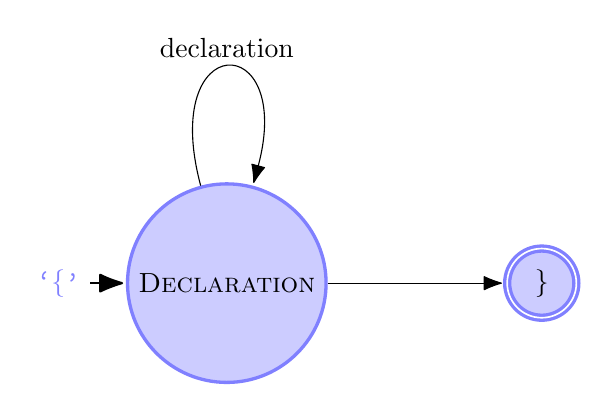
\begin{tikzpicture}[
        shorten >= 1pt, node distance = 4cm, on grid, 
        >= {Latex[round, scale = 1.5]},
        every state/.style = {draw = blue!50, very thick, fill = blue!20},
        every initial by arrow/.style = {text = blue!50, draw = black, thick}
    ]
      \node[state, initial, initial text = {\textbf{\texttt{`\{'}}}] (decl) {\textsc{Declaration}};
      \node[state, accepting] (end) [right = of decl] {\texttt{\textbf{\}}}};

      \path[->] 
        (decl) edge [loop above] node {declaration} (decl)
        (decl) edge node {} (end);
    \end{tikzpicture}
    \end{framed}


    \pagebreak

\section*{Expressions}

\begin{framed}
    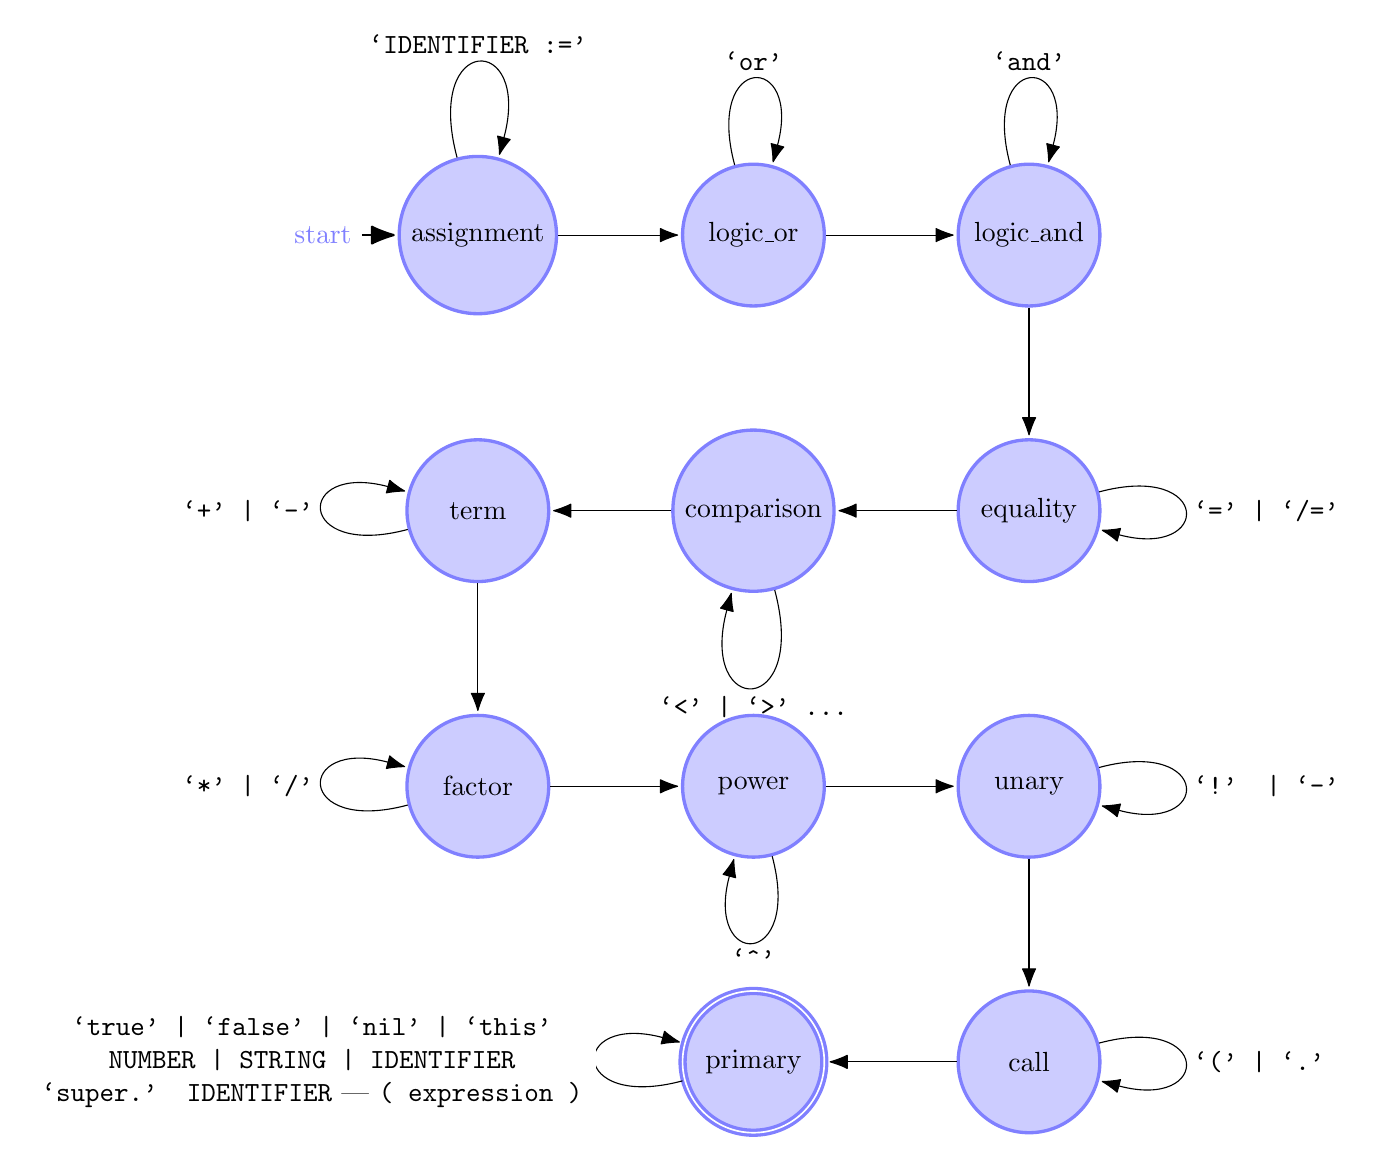
\begin{tikzpicture}[
        shorten >= 1pt, 
        node distance = 3.5cm,
        on grid, 
        >= {Latex[round, scale = 1.5]},
        every state/.style = {draw = blue!50, very thick, fill = blue!20, minimum size = 1.8cm},
        every initial by arrow/.style = {text = blue!50, draw = black, thick}
    ]

    \node[state, initial, initial where = left] (e0) {assignment};
    \node[state] (e1) [right = of e0] {logic\_or};
    \node[state] (e2) [right = of e1] {logic\_and};
    \node[state] (e3) [below = of e2] {equality};
    \node[state] (e4) [left = of e3] {comparison};
    \node[state] (e5) [left = of e4] {term};
    \node[state] (e6) [below = of e5] {factor};
    \node[state] (e7) [right = of e6] {power};
    \node[state] (e8) [right = of e7] {unary};
    \node[state] (e9) [below = of e8] {call};
    \node[state, accepting] (e10) [left = of e9] {primary};

    \path[->]
        (e0) edge node [above] {} (e1)
        (e1) edge node [above] {} (e2)
        (e2) edge node [right] {} (e3)
        (e3) edge node [above] {} (e4)
        (e4) edge node [above] {} (e5)
        (e5) edge node [left] {} (e6)
        (e6) edge node [above] {} (e7)
        (e7) edge node [above] {} (e8)
        (e8) edge node [right] {} (e9)
        (e9) edge node [above] {} (e10);

    \path[->]
        (e0) edge [loop above] node {\texttt{`IDENTIFIER :='}} (e0)
        (e1) edge [loop above] node {\texttt{`or'}} (e1)
        (e2) edge [loop above] node {\texttt{`and'}} (e2)
        (e3) edge [loop right] node {\texttt{`=' | `/='}} (e3)
        (e4) edge [loop below] node {\texttt{`<' | `>' \dots}} (e4)
        (e5) edge [loop left]  node {\texttt{`+' | `-'}} (e5)
        (e6) edge [loop left] node {\texttt{`*' | `/'}} (e6)
        (e7) edge [loop below] node {\texttt{`\^{}'}} (e7)
        (e8) edge [loop right] node {\texttt{`!' | `-'}} (e8)
        (e9) edge [loop right] node {\texttt{`(' | `.'}} (e9)
        (e10) edge [loop left, align=center] 
              node [fill=white, inner sep=5pt] {
                  \texttt{`true' | `false' | `nil' | `this'} \\ 
                  \texttt{NUMBER | STRING | IDENTIFIER} \\ 
                  \texttt{`super.' IDENTIFIER} | \texttt{( expression )}
              } (e10);
    \end{tikzpicture}
\end{framed}




\pagebreak


\section*{Functions}

\begin{framed}
    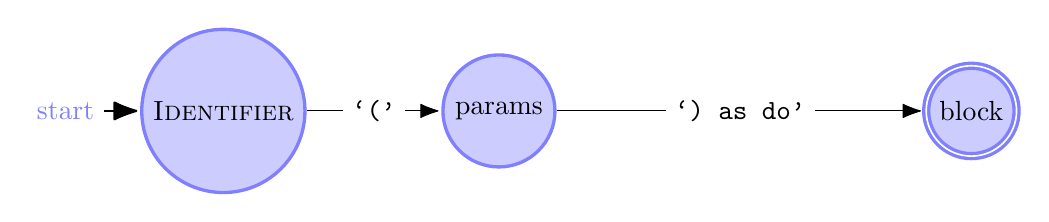
\begin{tikzpicture}[
        shorten >= 1pt, 
        node distance = 3.5cm,
        on grid, 
        >= {Latex[round, scale = 1.5]},
        every state/.style = {draw = blue!50, very thick, fill = blue!20},
        every initial by arrow/.style = {text = blue!50, draw = black, thick}
    ]



        \node[state, initial] (name) {\textsc{Identifier}};
        \node[state] (args) [right = of name] {params};
        \node[state, accepting] (block) [right = 6cm of args] {block};


        \path[->]
            (name) edge node [fill = white] {\textbf{\texttt{`('}}} (args)
            (args) edge node [fill = white] {\textbf{\texttt{`) as do'}}} (block);


    \end{tikzpicture}

\end{framed}



\section*{Parameters}

\begin{framed}
    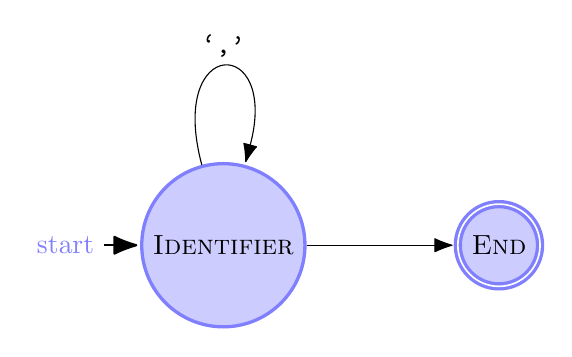
\begin{tikzpicture}[
        shorten >= 1pt, 
        node distance = 3.5cm,
        on grid, 
        >= {Latex[round, scale = 1.5]},
        every state/.style = {draw = blue!50, very thick, fill = blue!20},
        every initial by arrow/.style = {text = blue!50, draw = black, thick}
    ]


        \node[state, initial] (p1) {\textsc{Identifier}};
        \node[state, accepting] (s_e) [right = of p1] {\textsc{End}};
        
        \path[->]
            (p1) edge [loop above] node [] {\texttt{\textbf{`,'}}} (p1)
            (p1) edge node {} (s_e);



\end{tikzpicture}
\end{framed}



\section*{Arguments}

\begin{framed}
    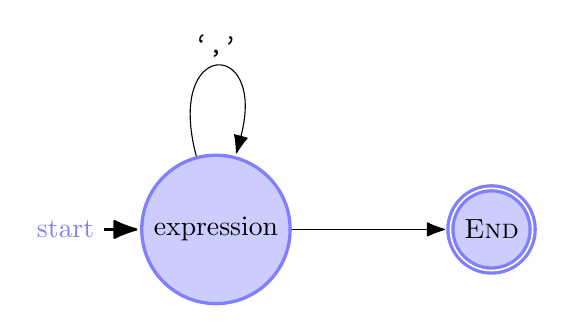
\begin{tikzpicture}[
        shorten >= 1pt, 
        node distance = 3.5cm,
        on grid, 
        >= {Latex[round, scale = 1.5]},
        every state/.style = {draw = blue!50, very thick, fill = blue!20},
        every initial by arrow/.style = {text = blue!50, draw = black, thick}
    ]

        \node[state, initial] (s1) {expression};
        \node[state, accepting] (s_e) [right = of s1] {\textsc{End}};
        
        \path[->]
            (s1) edge [loop above] node [] {\texttt{\textbf{`,'}}} (s1)
            (s1) edge node {} (s_e);




    \end{tikzpicture}

\end{framed}


\end{center}

\pagebreak



\section*{Lexical Grammar}


\begin{itemize}

    \item \textsc{Number}         $\rightarrow$ \textsc{Digit}\textbf{\texttt{+}} (\textbf{\texttt{`.'}} \textsc{Digit}\textbf{\texttt{+}})\textbf{\texttt{?}};
    \item \textsc{String}         $\rightarrow$ \texttt{\textbf{`"' [\^{}"]* `"'}};
    \item \textsc{Identifier}     $\rightarrow$ \textsc{Char} (\textsc{Char} | \textsc{Digit})\texttt{\textbf{*}};
    \item \textsc{Char}           $\rightarrow$ \texttt{\textbf{`a'..'z' | `A'..`Z' | `\_{}'}};
    \item \textsc{Digit}          $\rightarrow$ \texttt{\textbf{`0'..`9'}};

\end{itemize}




\end{document}




